\section{Introduction}\label{sec:introduction}

Linear attention, which compresses the token history into a fixed-size recurrent state, is now widely used in long-context large language models.
For instance, recent hybrid architectures in the Qwen, Kimi, and GLM model families replace many standard attention layers with recurrent linear attention layers such as Gated DeltaNet (GDN) and Kimi Delta Attention (KDA)~\citep{qwen2025qwen3next,yang2025gated,team2025kimi}.
By compressing the token history, these layers reduce the computation and memory growth associated with long context, making inference more efficient.

However, the recurrent state in linear attention still imposes substantial memory bandwidth and capacity costs during inference.
For each generated token, a linear-attention layer loads its state matrix from HBM, applies a lightweight update, computes the token output, and writes the updated matrix back to HBM.
This full-state transfer repeats at every decoding step.
Since the update and readout perform little arithmetic relative to the bytes transferred, inference throughput is bottlenecked by HBM bandwidth~\citep{williams2009roofline}.
Consequently, reading and writing the recurrent states across many linear attention layers and concurrent requests accounts for a significant fraction of decoding time, as shown in Figure~\ref{fig:intro}(a).
Additionally, the recurrent state consumes substantial GPU memory when prefix caching is enabled, as serving systems retain separate states for each cached prefix (Figure~\ref{fig:intro}(b))~\citep{pan2025marconi}.
\begin{figure}[t]
    \centering
    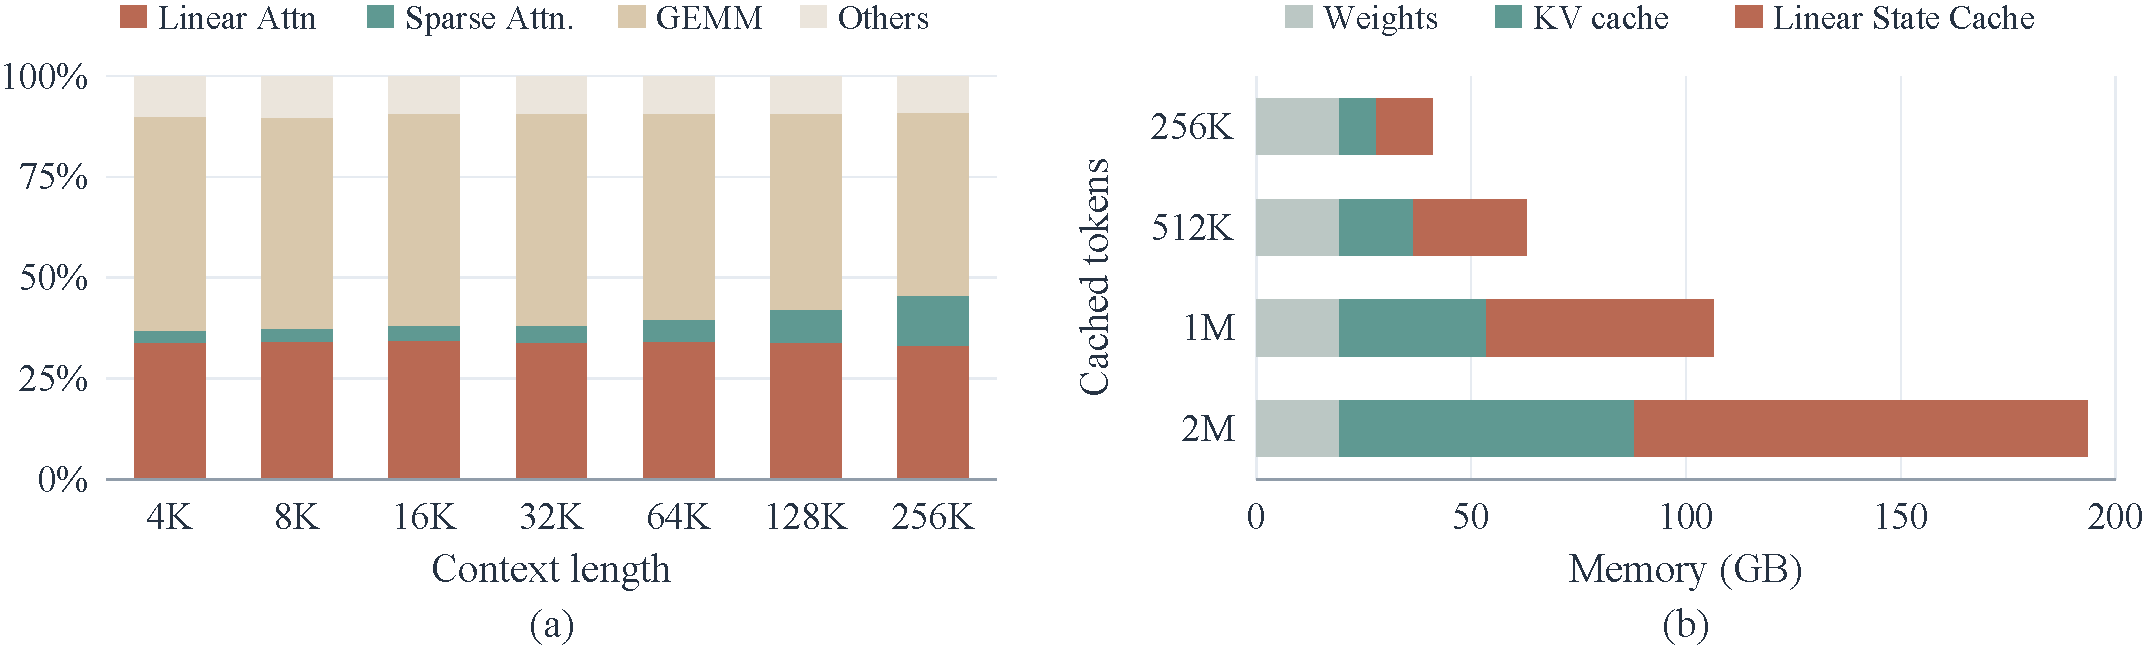
\includegraphics[width=\linewidth]{figures/intro_serving_cost.pdf}
    \caption{Recurrent-state access is a major cost of LLM serving.
    (a) Decode-time breakdown for GLM-5.3-Flash-NVFP4 on the B200 GPU at batch size 256. The share spent on linear attention stays roughly constant as context length grows.
    (b) GPU memory footprint for Qwen3.5-9B with prefix caching, assuming one linear attention state per 1{,}024 cached tokens.}
    \vspace{-1em}
    \label{fig:intro}
\end{figure}


Quantizing the recurrent state is a natural way to reduce both memory traffic and footprint, but doing so in a way that preserves model accuracy is challenging.
In particular, a naive approach that stores the state in a standard low-bit format and re-quantizes it after every token can substantially degrade accuracy, especially over long thinking traces.
We find that accuracy degradation arises from two sources of error.
First, quantization error accumulates recurrently: each update starts from an already quantized state, and quantizing the result introduces another rounding error, causing the state to deviate progressively from the FP32 trajectory over a long generation (Figure~\ref{fig:state-error}).
Second, large outliers are often concentrated in a few rows and columns of the state.
These outliers widen the quantization range and force smaller values onto coarse quantization levels, amplifying the error introduced each time the state is quantized.
Accurate low-bit quantization therefore requires reducing both how often error is introduced and how much error each quantization introduces.

We propose \emph{\sys{}}, a training-free method for recurrent-state quantization that achieves near-lossless model quality.
\sys{} introduces two key ideas that directly address the above sources of error.
First, \emph{per-window quantization} limits error accumulation by allowing \sys{} to \emph{leap} over a window of tokens before quantizing the state again (Figure~\ref{fig:per-window}).
At the beginning of each window, \sys{} stores the recurrent state in low precision.
Within the window, it holds this state fixed, buffers higher-precision token updates, and computes each output from the fixed state and buffered updates.
Only at the end of the window does it reconstruct and quantize the full updated state for the next window.
As a result, \sys{} introduces quantization error less frequently, slowing its accumulation over long contexts.

To address quantization error caused by outliers, \sys{} introduces \emph{Compensator Tokens}, which capture the state's largest outliers in high precision and thereby reduce the error of each quantization (Figure~\ref{fig:ghost-tokens}).
Each Compensator Token represents a high-precision outer product of two vectors, capturing large-magnitude patterns across both rows and columns and leaving a residual that is easier to quantize.
Since these rank-one terms have the same form as real-token updates, \sys{} incorporates them directly into the window's update path using only a few additional vectors and no separate recurrent state update.
\sys{} further smooths the residual across channels before quantization to reduce error.
Both key techniques in \sys{} are training-free and require no calibration data.

Our evaluation spanning the Qwen, Kimi, and GLM families demonstrates that \emph{\sys{}} substantially reduces memory costs and improves inference throughput.
Across 12 model--task pairs, \sys{} achieves accuracy comparable to the FP32 baseline while reducing state memory traffic by 3.4$\times$ and end-to-end memory footprint by up to 56\%.
Across NVIDIA B200, RTX PRO 6000, and RTX 5090 GPUs, \sys{} achieves average speedups of 2.05--3.70$\times$ at the kernel level and 1.47$\times$ for end-to-end inference.

\begin{figure}[t]
    \centering
    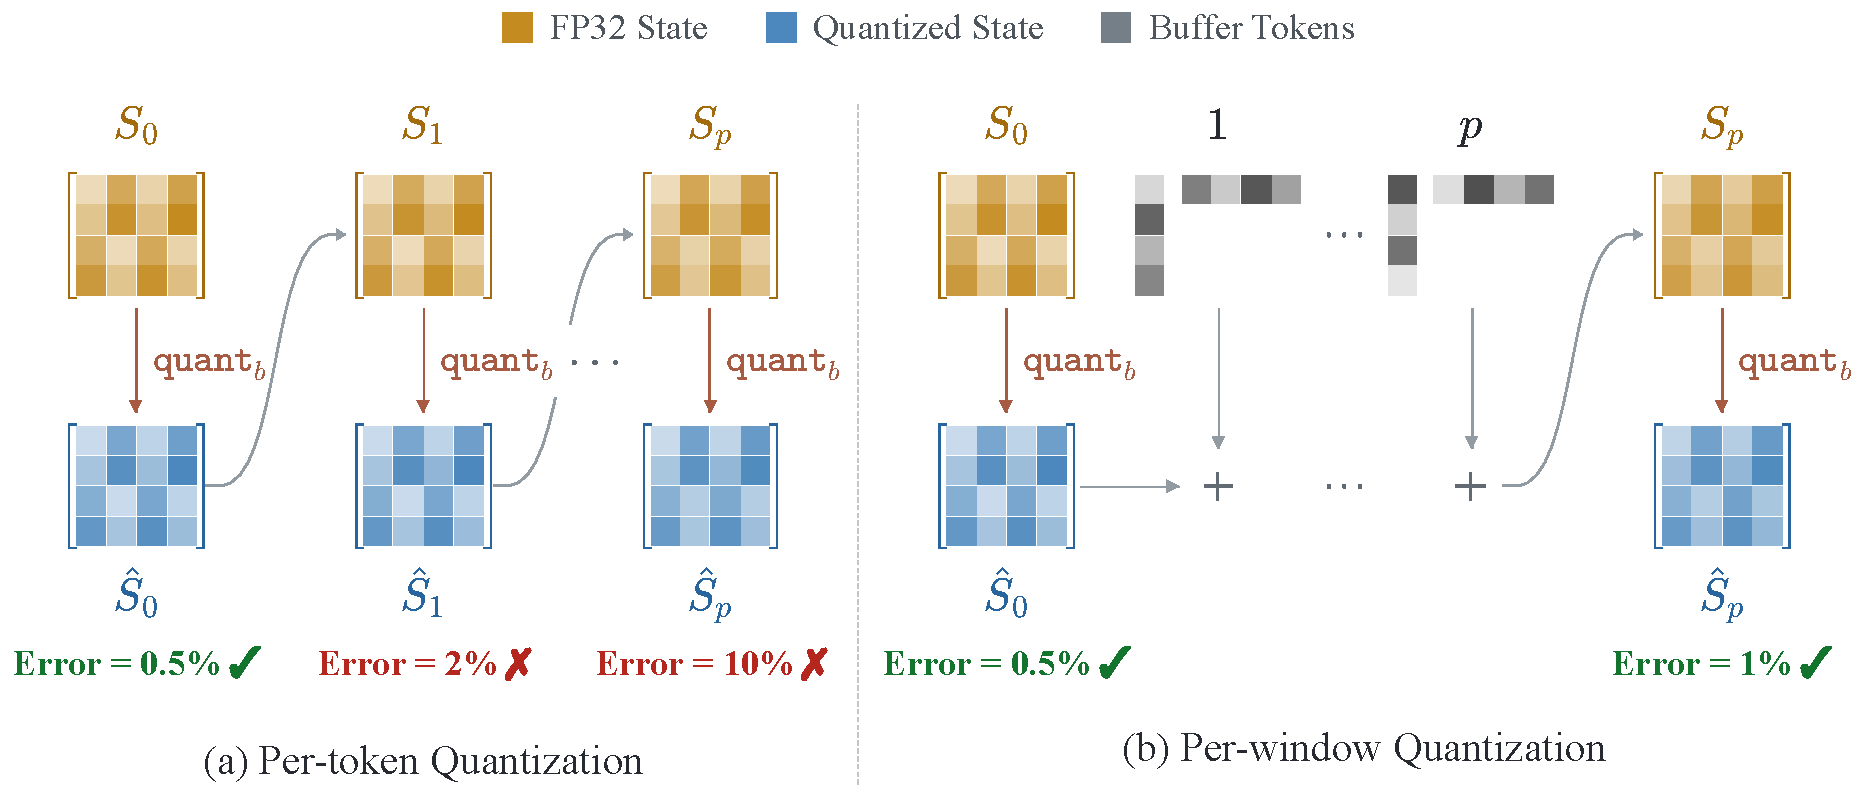
\includegraphics[width=0.9\linewidth]{figures/per-window-quantization-paper.pdf}
    \caption{Per-token versus per-window quantization. Per-token quantization re-quantizes the full state after every update. Per-window quantization holds the quantized boundary state $\hat S_0$ fixed, buffers the $p$ updates of the window in higher precision, and reconstructs the state from them; the full state is quantized only once per window, into $\hat S_p$.}
    \label{fig:per-window}
    \vspace{-1.5em}
\end{figure}

